\documentclass[10pt,a4paper]{article}
\usepackage[utf8]{inputenc}
\usepackage[T1]{fontenc}
\usepackage{amsmath}
\usepackage{amsfonts}
\usepackage{amssymb}
\usepackage{hyperref}
\usepackage{graphicx}
\usepackage{float}
\usepackage{pythonhighlight}
\usepackage{listings}
\usepackage[english]{babel}
\usepackage{subfig}
\newcommand{\figura}[3][0.95]{
	\begin{figure}[H]
		\centering
		\includegraphics[width=#1\linewidth]{#2}
		\caption{#3}
		\label{fig::#2}
	\end{figure}
}
\begin{document}
\selectlanguage{english}
\begin{center}
	Advanced Topics in Numerical Methods for Partial Differential Equations\\
	
	\vspace{5pt}
	
	16.930
	
	\vspace{10pt}
	
	Massachusetts Institute of Technology
	
	\vspace{170pt}
	
	\Large{\textsc{Project 5 - HDG for the Convection-Diffusion Equation}}
	
	\vspace{20pt}
	
	Renato Trono Figueras
	
	\vspace{20pt}
	
	May 2023
\end{center}
\newpage

\section*{HDG Formulation for the Convection-Diffusion Problem}

The objective of this project is to extend the code by implementing the Hybridizable Discontinuous Galerkin (HDG)
method to solve the 2D convection-diffusion equation. First, we look at the formulation of the problem, and then we briefly summarize the implementation aspects.
\subsection*{Strong Form of the Equation}

We are interested in solving the following system of equation:

\begin{equation}
    \mathbf{q} - \nabla u = \mathbf{0},~~~\text{in}~ \Omega 
\end{equation}

\begin{equation}
    -\nabla \cdot (\kappa \mathbf{q}) + \nabla \cdot (\mathbf{c}u) = f,~~~\text{in}~\Omega 
\end{equation}

\begin{equation}
    u = g,~~~\text{on}~\partial \Omega
\end{equation}
where $\Omega \subset \mathbb{R}^d$, with $d$ the spatial dimension of the problem ($d = 2$ in this case).
\subsection*{Approximation Spaces}

We now introduce the approximation spaces for the computed solutions using the HDG method:

\begin{equation}
    u_h \in W_h^k,~~~W_h^k := \{w \in L^2(\mathcal{T}_h) : w|_K \in \mathcal{P}_k(K),~\forall K \in \mathcal{T}_h \}
\end{equation}

\begin{equation}
    \mathbf{q}_h \in \mathbf{V}_h^k,~~~\mathbf{V}_h^k := \{\mathbf{v} \in [L^2(\mathcal{T}_h)]^d : \mathbf{v}|_K \in [\mathcal{P}_k(K)]^d,~\forall K \in \mathcal{T}_h \}
\end{equation}

\begin{equation}
    \hat{u}_h \in M_h^k,~~~M_h^k : = \{\mu \in L^2(\mathcal{E}_h) : \mu|_F \in \mathcal{P}_k(F),~\forall F \in \mathcal{E}_h \}
\end{equation}
where $\mathcal{T}_h$ is the triangulation, $K$ refers to element $K$, $\mathcal{P}_k$ is the space of polynomials up to degree $k$,
$\mathcal{E}_h$ is the set of faces, and $F$ refers to face $F$.

\subsection*{Weak formulation}

For the weak formulation of the problem, we consider each element separately on the one hand, and each faces separately on the other hand. 
Hence, for element $K$, if we know the value of the solution on $\partial K$, say $\hat{u}$, we can solve for the solution in the interior of element $K$; this is known as the
local problem.
On the other hand, we also need to solve for $\hat{u}$ on all the faces of $\mathcal{T}_h$, which is known as the global problem.
Let's see in more detail the local and global problems.
\subsubsection*{Local problem}

The weak formulation of the local problem in element $K$ is as follows. 
Given $\hat{u}_h$, which is an approximation for $\hat{u}$ on $\partial K$, find $(\mathbf{q}_h,u_h) \in [\mathcal{P}_k(K)]^d \times \mathcal{P}_k(K)$ such that:

\begin{equation}
    (\kappa^{-1}\mathbf{q}_h,\mathbf{v})_K + (u_h,\nabla \cdot \mathbf{v})_K - \left<\hat{u}_h,\mathbf{v}\cdot \mathbf{n}\right>_{\partial K} = 0,~~~\forall \mathbf{v} \in [\mathcal{P}_k(K)]^d
	\label{e:local1}
\end{equation}

\begin{equation}
    (\mathbf{q}_h,\nabla w)_K - (\mathbf{c}u_h,\nabla w)_K
    - \left<\mathbf{q} \cdot \mathbf{n},w\right>_{\partial K}
    + \left<(\mathbf{c}\cdot\mathbf{n} - \tau)\hat{u}_h,w\right>_{\partial K}
    + \left<\tau u_h,w\right>_{\partial K} = (f,w)_K,~ \forall w \in \mathcal{P}_k(K)
\end{equation}
where $\tau > 0$ is the stabilization parameter.

\subsubsection*{Global problem}

The global problem solves for $\hat{u}_h$, imposing the boundary
conditions and the jump condition for the flux across elements. In particular; find $\hat{u}_h \in M_h^k$ such that:

\begin{equation}
	\left<\hat{\mathbf{f}}_h \cdot \mathbf{n}, \mu\right>_{\partial \mathcal{T}_h \setminus \partial \Omega}
	+ \left<\hat{u}_h - g_D, \mu\right>_{\partial \Omega_D} 
	+ \left<\hat{\mathbf{f}}_h \cdot \mathbf{n} - g_N, \mu \right>_{\partial \Omega_N} = 0,~\forall \mu \in M_h^k
	\label{e:global}
\end{equation}
where $\hat{\mathbf{f}}_h = \mathbf{q}_h - \mathbf{c}\hat{u} - \tau(u_h - \hat{u}_h)\mathbf{n}$.
\subsubsection*{Complete formulation and matricial form}

The discretization of weak formulation for the local and global problems leads to the following matricial form:

\begin{equation}
	\begin{bmatrix}
		A & B & C \\
		-B^T & D & -E \\
		C^T & - E^T & M
	\end{bmatrix}
	\begin{bmatrix}
		U \\
		Q \\
		\hat{U}
	\end{bmatrix}
	=
	\begin{bmatrix}
		\mathbf{0} \\
		F\\
		G
	\end{bmatrix}
\end{equation}
where the matrix:

\begin{equation}
	\begin{bmatrix}
		A & B \\
		-B^T & D
	\end{bmatrix}
\end{equation}
is block-diagonal and invertible if $\tau > 0$. and where $U$, $Q$ and $\hat{U}$ are the vectors of
unknowns for $u_h$ $\mathbf{q}_h$ ($Q = [Q_x,Q_y]^T$), and $\hat{u}$, respectively.  
Hence, we can eliminate $U$ and $Q$ and form the following system for $\hat{U}$:

\begin{equation}
	H\hat{U}=R
\end{equation}
where:

\begin{equation}
	H 
	=
	M 
	+ 
	\begin{bmatrix}
		C^T & -E^T
	\end{bmatrix}
	\begin{bmatrix}
		A & B \\
		-B^T & D
	\end{bmatrix}^{-1}
	\begin{bmatrix}
		C \\
		E
	\end{bmatrix}
\end{equation}

\begin{equation}
	R
	=
	G 
	-
	\begin{bmatrix}
		C^T & -E^T
	\end{bmatrix}
	\begin{bmatrix}
		A & B \\
		-B^T & D
	\end{bmatrix}^{-1}
	\begin{bmatrix}
		\mathbf{0} \\
		F
	\end{bmatrix}
\end{equation}
where all the matrices and vectors are built according to the different terms in 
Eqs. \ref{e:local1} - \ref{e:global}.

Once the global problem is solved, the local problem on each element can be solved to finally get the complete solution of the problem.
\subsection*{Local Postprocessing}

Due to the way we solve the problem, both $u_h$ and $\mathbf{q}_h$ are approximated with polynomials of the same order, and so the solutions are of the same order. Hence, since $\mathbf{q} = \nabla u$, we can
integrate $\mathbf{q}_h$ to obtain a better solution for $u$ than it is $u_h$, name it $u^*_h$. This process is known as local postprocessing. In particular, we want
$u^*_h \in \mathcal{P}_{k+1}(K)$ such that on every element $K \in \mathcal{T}_h$:

\begin{equation}
	(\kappa \nabla u^*_h, \nabla w)_K = (\mathbf{q}_h,\nabla w)_K,~~~ \forall w \in \mathcal{P}_{k+1}(K)
\end{equation}

\begin{equation}
	(u^*_h,1)_K = (u_h,1)_K
\end{equation}
where the second condition is imposed to avoid a singular system, since the problem is a pure Neumann problem.

\subsection*{Implementation Aspects}

The extension of the code consists essentially on three new functions: \textit{localprob()}, \textit{hdg\_solve} and \textit{hdg\_postprocess}.
The function \textit{localprob()} was already given, and was slightly modified to allow for different values of $\tau$ for interior or boundary faces. What this function does is to solve the local problem
for an element, given $\hat{u}_h$ on its boundary, and given $F$.

On the other hand, \textit{hdg\_solve} solves first the global problem, and then uses its solution to call \textit{localprob()} for each element, computing then the complete solution.

Finally, the output of \textit{hdg\_solve} is passed to \textit{hdg\_postprocess}, which recover $u^*_h$ by performing the local postprocessing explained in the pervious subsection.
\section*{Convergence Study for the Diffusion Problem}
We first tested the implementation on the pure diffusion equation (i.e. $\mathbf{c} = \mathbf{0}$) with homogeneous Dirichlet boundary conditions. For this,
we used the unit square domain, and set the source term $f$ such that the exact solution is:

\begin{equation}
	u(x,y) = \sin(\pi x)\sin(\pi y)
\end{equation}

We used three different values for the stabilization parameter $\tau$: $1$, $h$ and $1/h$, where $h$ is a measure of the element size.
The $L_2$ norm the errors for $u_h$, $\mathbf{q}_h$ and $u^*_h$ are shown in Figs. \ref{f:conv_tau_1} - \ref{f:conv_tau_h}, for the different $\tau$ cases.
\begin{figure}[H]
    \centering
    \subfloat[$u_h$.]{
        \label{f:square_straight}
        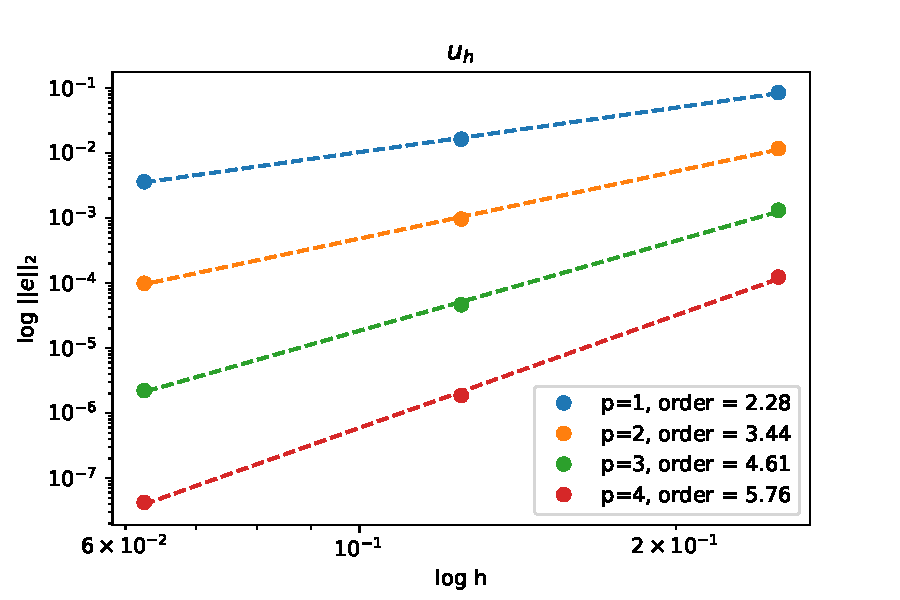
\includegraphics[width=0.33\textwidth]{uh_1.pdf}}
    \subfloat[$\mathbf{q}_h$.]{
        \label{f:square_distorted}
        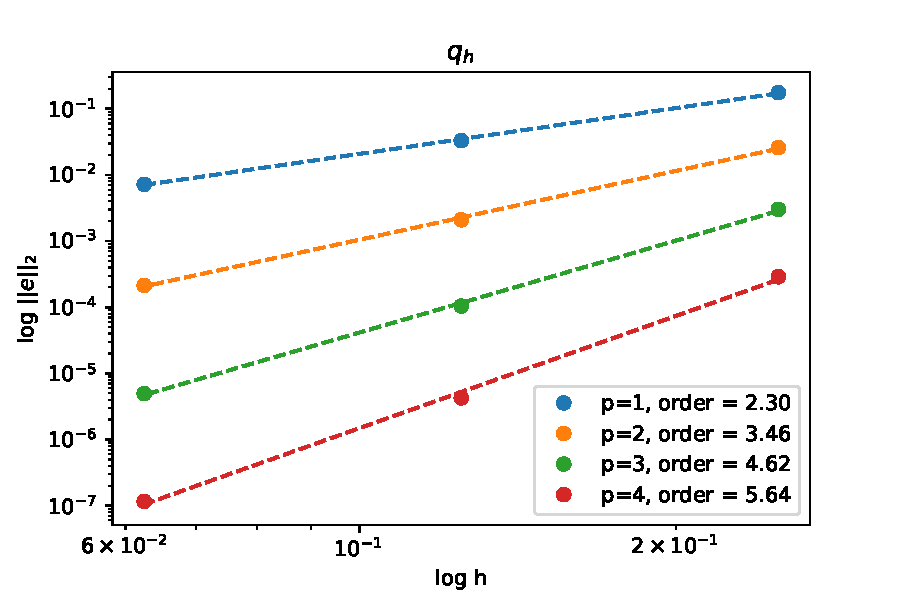
\includegraphics[width=0.33\textwidth]{qh_1.pdf}}
	\subfloat[$u^*_h$.]{
		\label{f:square_distorted}
		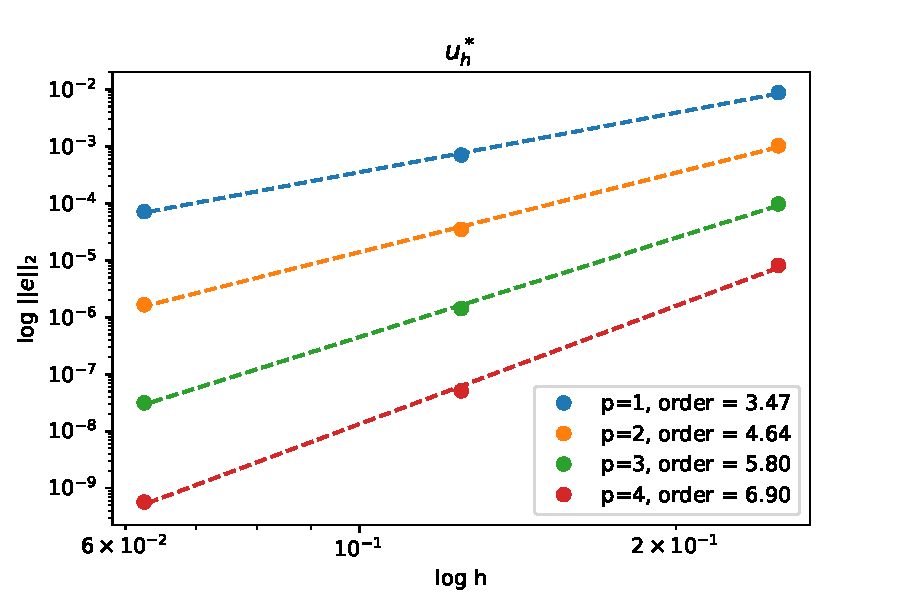
\includegraphics[width=0.33\textwidth]{ustarh_1.pdf}}
    \caption{$\tau = 1$}
    \label{f:conv_tau_1}
\end{figure}

\begin{figure}[H]
    \centering
    \subfloat[$u_h$.]{
        \label{f:square_straight}
        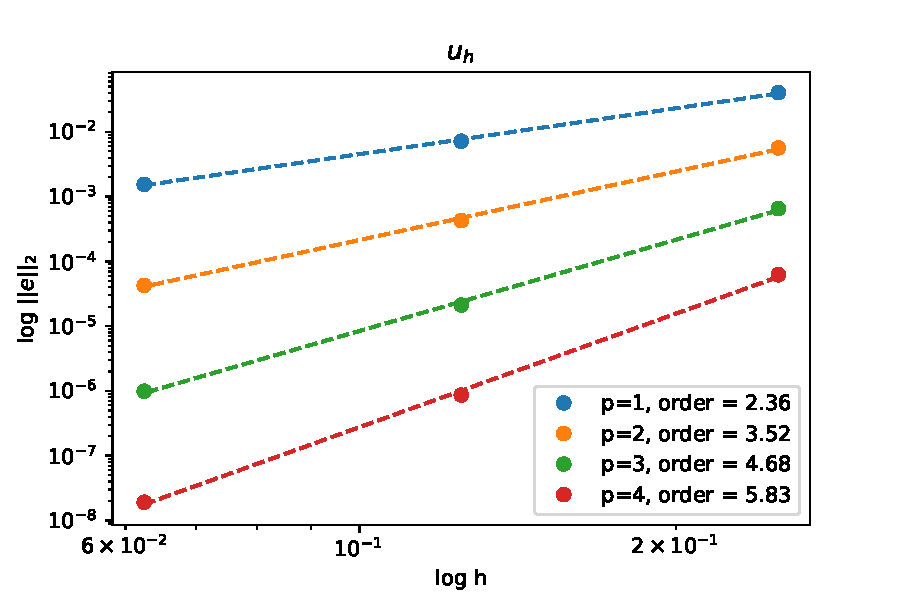
\includegraphics[width=0.33\textwidth]{uh_1_h.pdf}}
    \subfloat[$\mathbf{q}_h$.]{
        \label{f:square_distorted}
        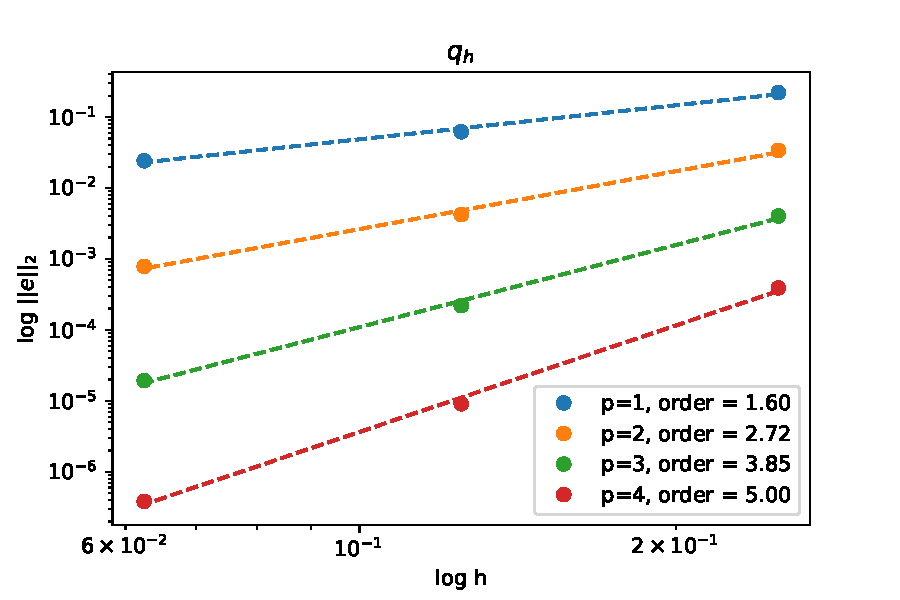
\includegraphics[width=0.33\textwidth]{qh_1_h.pdf}}
	\subfloat[$u^*_h$.]{
		\label{f:square_distorted}
		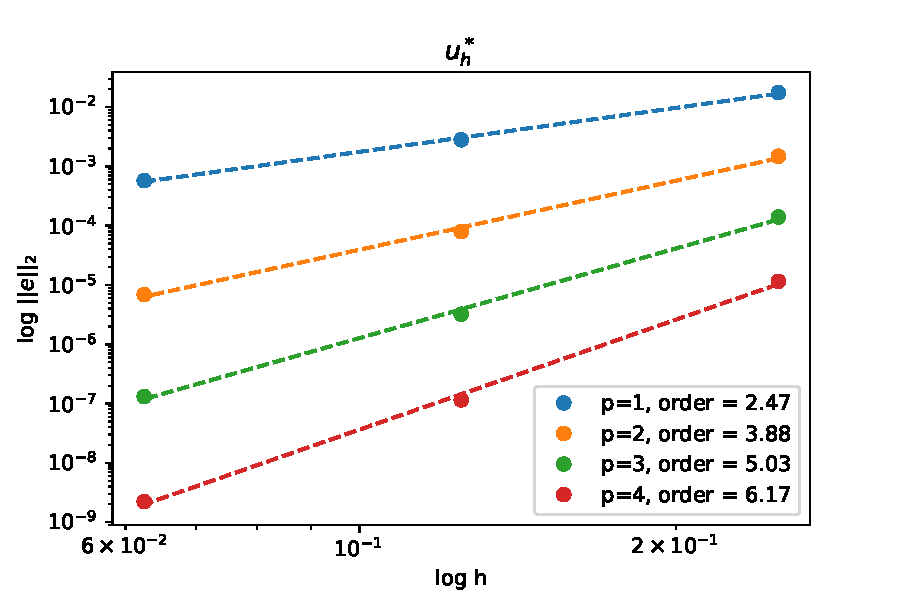
\includegraphics[width=0.33\textwidth]{ustarh_1_h.pdf}}
    \caption{$\tau = 1/h$.}
    \label{f:u_scattered}
\end{figure}

\begin{figure}[H]
    \centering
    \subfloat[$u_h$.]{
        \label{f:square_straight}
        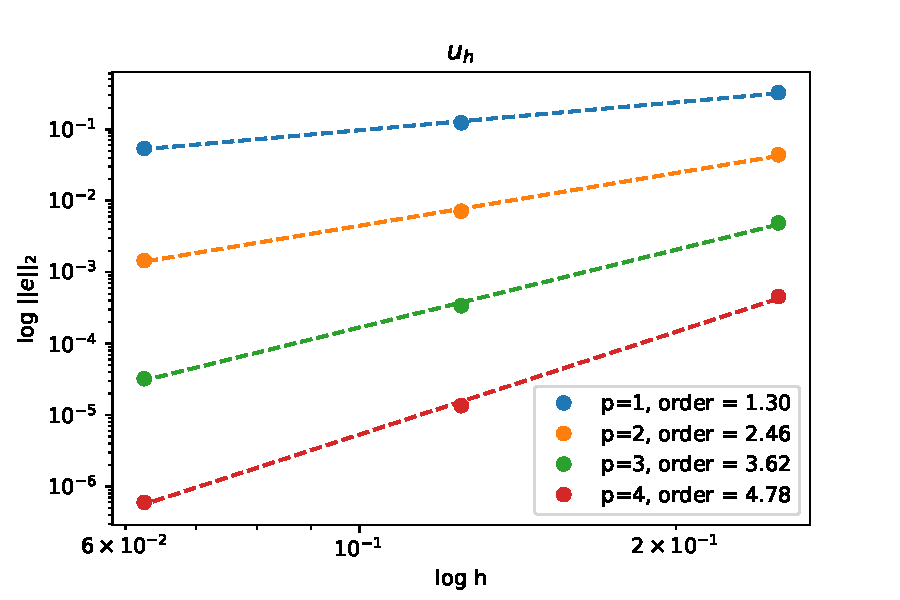
\includegraphics[width=0.33\textwidth]{uh_h.pdf}}
    \subfloat[$\mathbf{q}_h$.]{
        \label{f:square_distorted}
        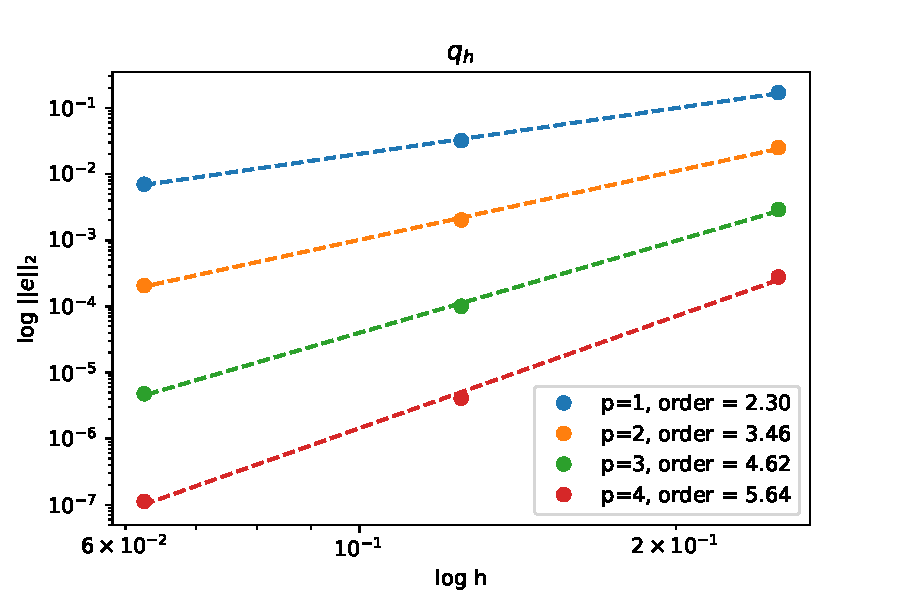
\includegraphics[width=0.33\textwidth]{qh_h.pdf}}
	\subfloat[$u^*_h$.]{
		\label{f:square_distorted}
		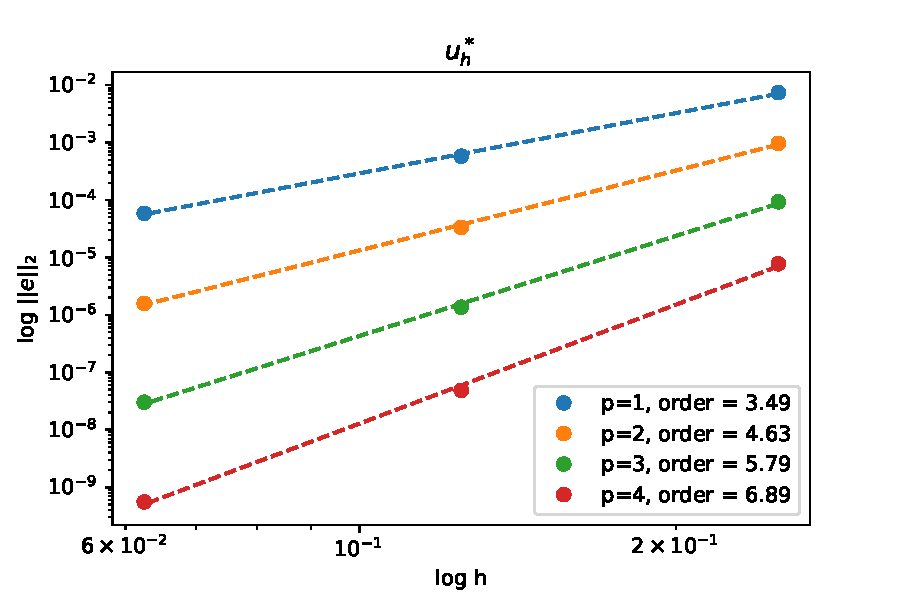
\includegraphics[width=0.33\textwidth]{ustarh_h.pdf}}
    \caption{$\tau = h$.}
    \label{f:conv_tau_h}
\end{figure}
For the case $\tau = 1$, we obtain optimal convergence for $u_h$ and $\mathbf{q}_h$ (i.e. $p+1$), and superconvergence for $u^*_h$ (at least $p+2$).
For the case $\tau = 1/h$, we obtain optimal convergence for $u_h$ but not for $\mathbf{q}_h$ on the lower orders. Hence, for the lower orders we do not obtain superconvergence for $u^*_h$ either,
although we obtain superconvergence for $p = 3$ and $p=4$. Finally, for the case $\tau = h$ we do not obtain optimal convergence for $u_h$, but we do for $\mathbf{q}_h$. Therefore, since $u^*_h$ is obtained from $\mathbf{q}_h$, we get superconvergence for $u^*_h$.

\section*{Comparison between the HDG solution and the Postprocessed Solution
for the Convection-Diffusion Problem}

Secondly, we tested the implementation with the convection-diffusion problem, for three cases:
diffusion-dominant $\mathbf{c} = (1,1)$, convection diffusion $\mathbf{c} = (10,10)$, and convection dominant $\mathbf{c} = (100,100)$. In particular, we compared the solution
$u_h$ with the postprocessed solution $u^*_h$ for curved meshes and different grid sizes on each case, using again the unit square domain with homogeneous Dirichlet boundary conditions, and using $f=10$. Also, the 
stabilization parameter used was $\tau = 1 + |\mathbf{c} \cdot \mathbf{n}|$.
The results are shown in Figs. \ref{f:conv_diff_1}-\ref{f:conv_diff_3}.

\begin{figure}[H]
    \centering
    \subfloat[$u_h$.]{
        \label{f:square_straight}
        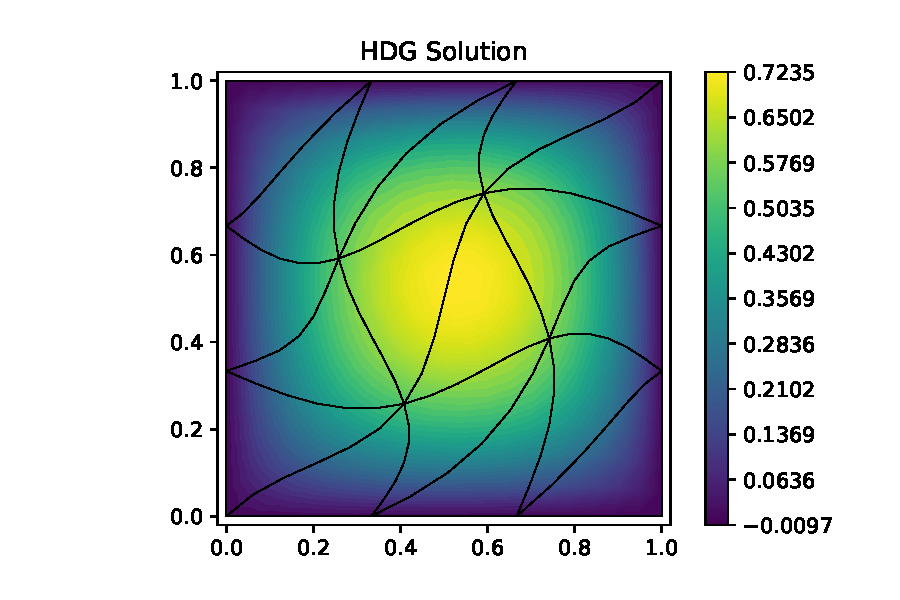
\includegraphics[width=0.5\textwidth]{uh_c_1.0_4.pdf}}
    \subfloat[$u^*_h$.]{
        \label{f:square_distorted}
        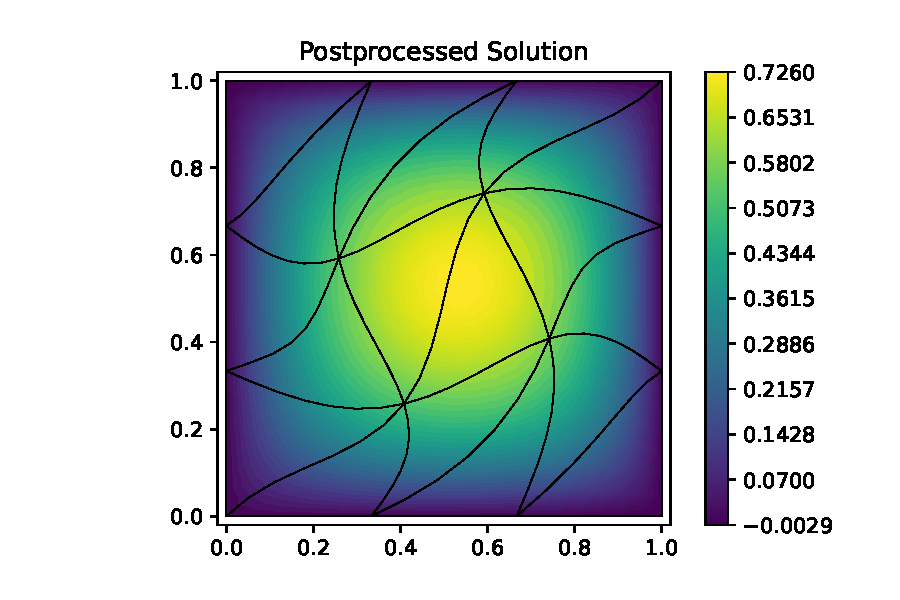
\includegraphics[width=0.5\textwidth]{ustarh_c_1.0_4.pdf}}\\
	\subfloat[$u_h$.]{
		\label{f:square_distorted}
		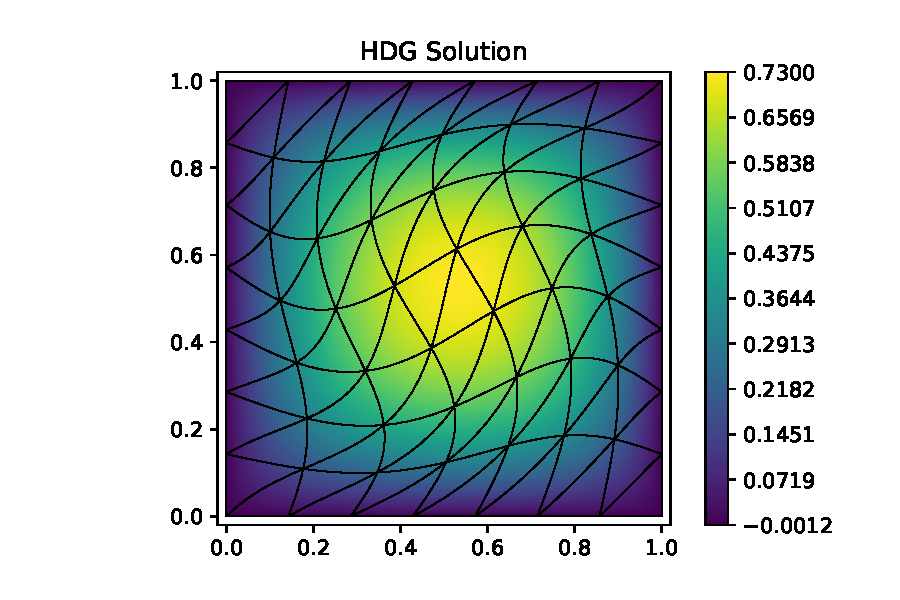
\includegraphics[width=0.5\textwidth]{uh_c_1.0_8.pdf}}
	\subfloat[$u^*_h$.]{
		\label{f:square_distorted}
		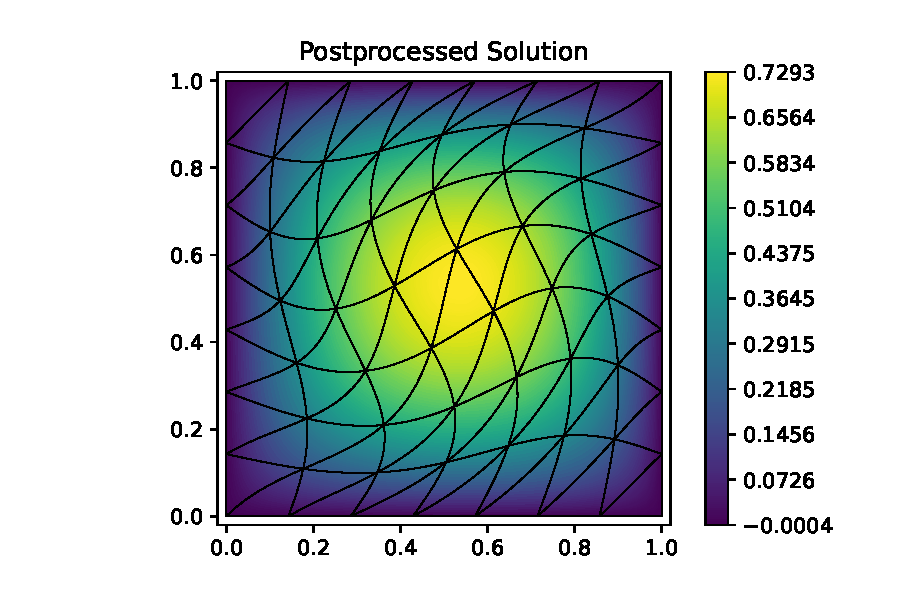
\includegraphics[width=0.5\textwidth]{ustarh_c_1.0_8.pdf}}\\
	\subfloat[$u_h$.]{
		\label{f:square_distorted}
		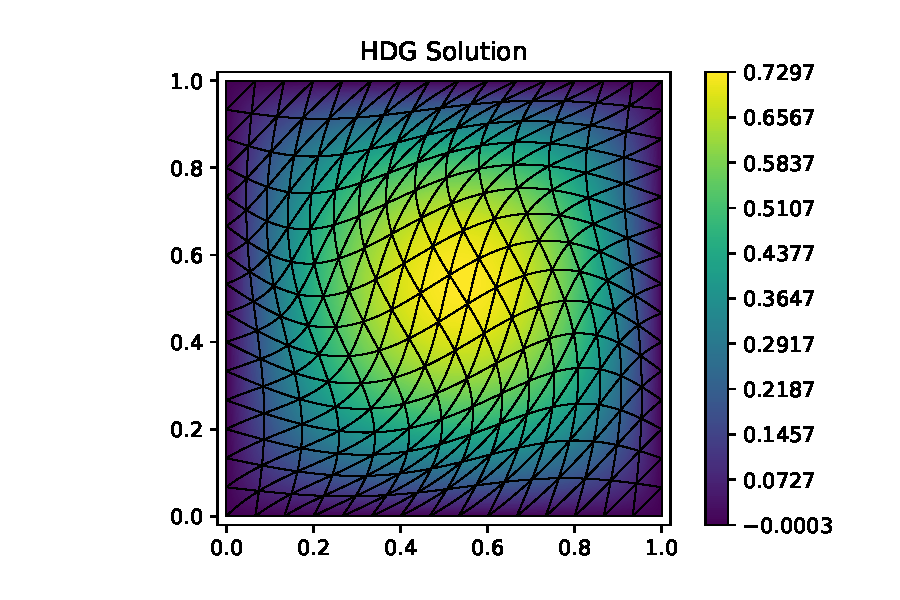
\includegraphics[width=0.5\textwidth]{uh_c_1.0_16.pdf}}
	\subfloat[$u^*_h$.]{
		\label{f:square_distorted}
		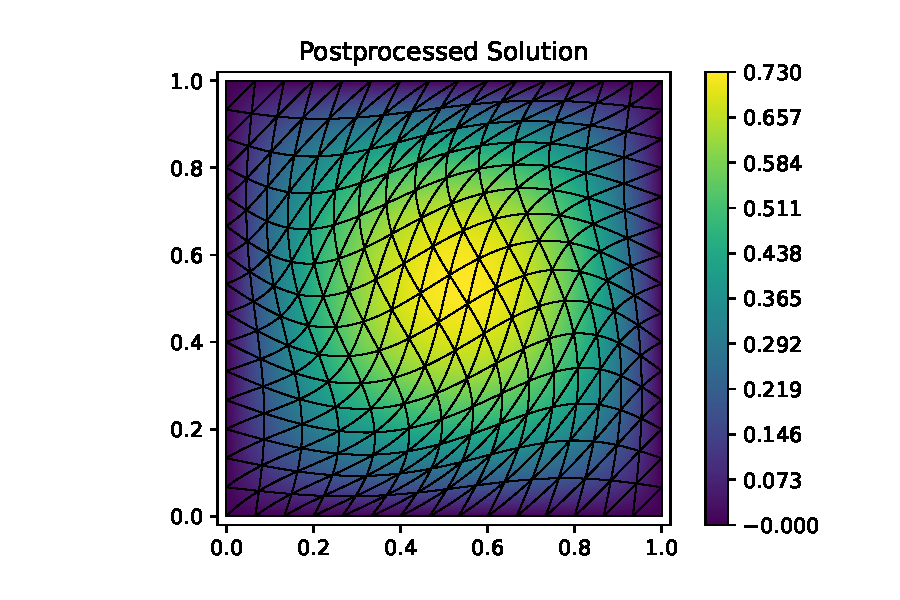
\includegraphics[width=0.5\textwidth]{ustarh_c_1.0_16.pdf}}
    \caption{$\mathbf{c}= (1,1)$}
    \label{f:conv_diff_1}
\end{figure}

\begin{figure}[H]
    \centering
    \subfloat[$u_h$.]{
        \label{f:square_straight}
        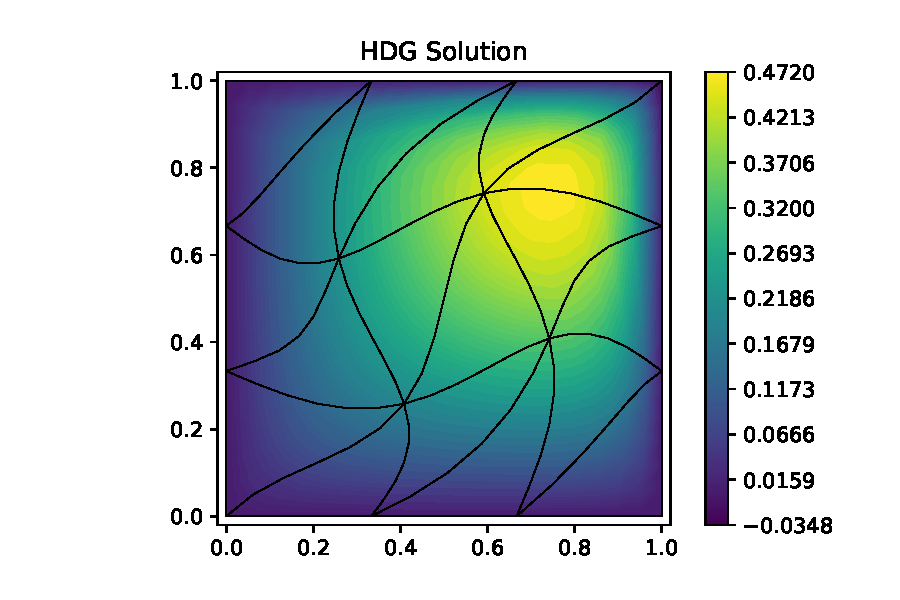
\includegraphics[width=0.5\textwidth]{uh_c_10_4.pdf}}
    \subfloat[$u^*_h$.]{
        \label{f:square_distorted}
        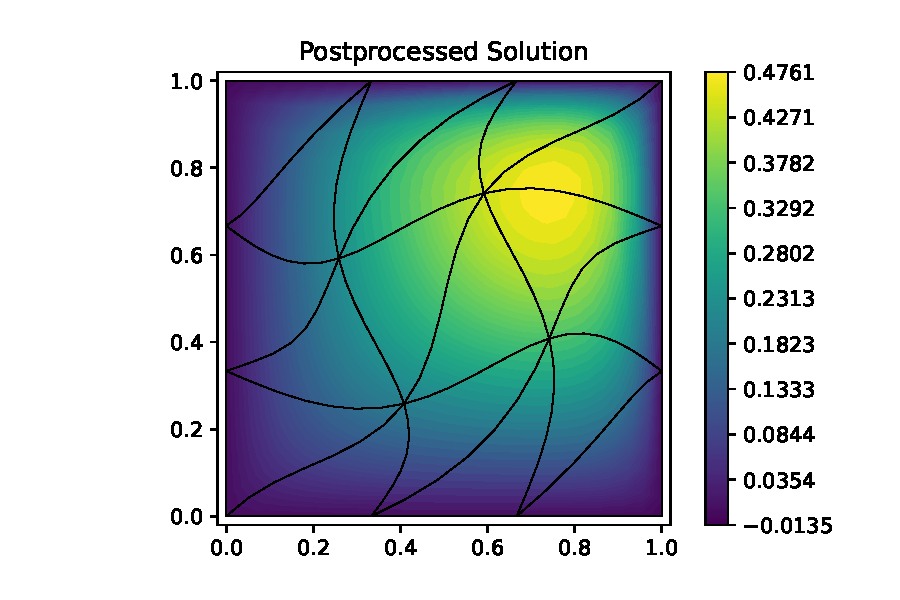
\includegraphics[width=0.5\textwidth]{ustarh_c_10_4.pdf}}\\
	\subfloat[$u_h$.]{
		\label{f:square_distorted}
		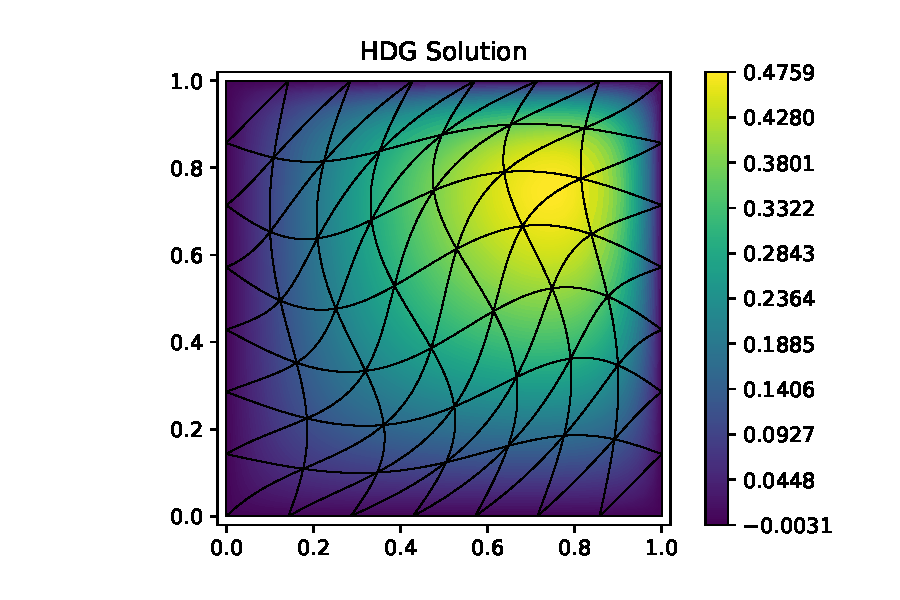
\includegraphics[width=0.5\textwidth]{uh_c_10_8.pdf}}
	\subfloat[$u^*_h$.]{
		\label{f:square_distorted}
		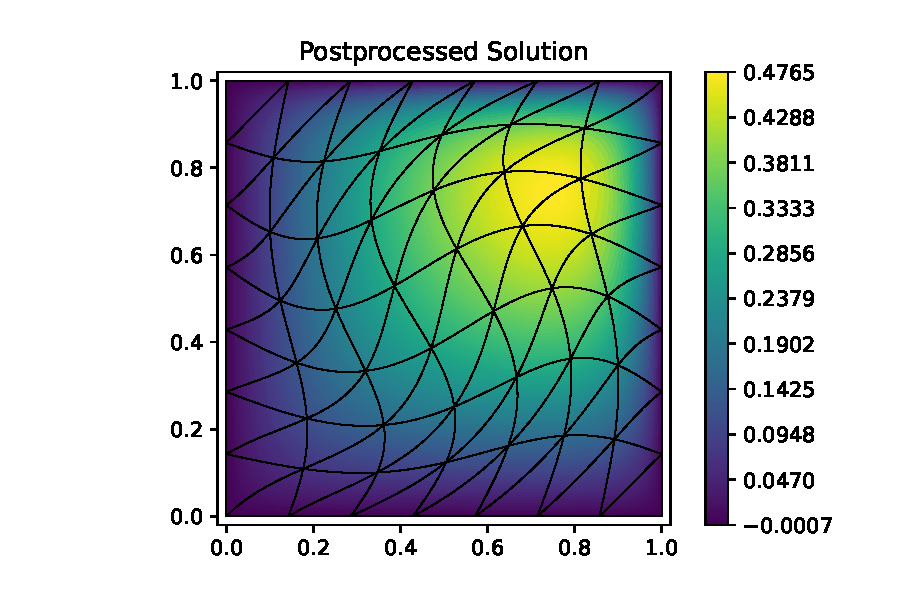
\includegraphics[width=0.5\textwidth]{ustarh_c_10_8.pdf}}\\
	\subfloat[$u_h$.]{
		\label{f:square_distorted}
		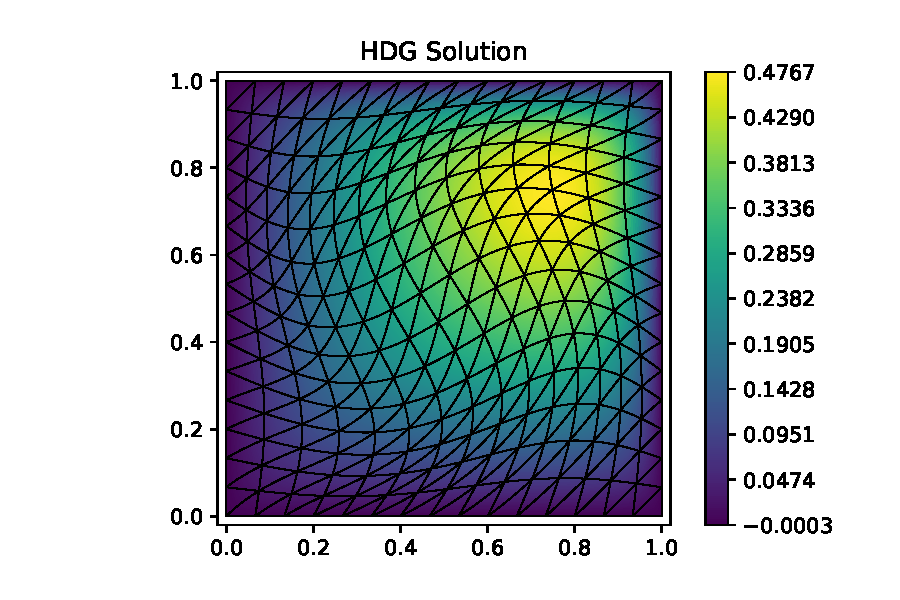
\includegraphics[width=0.5\textwidth]{uh_c_10_16.pdf}}
	\subfloat[$u^*_h$.]{
		\label{f:square_distorted}
		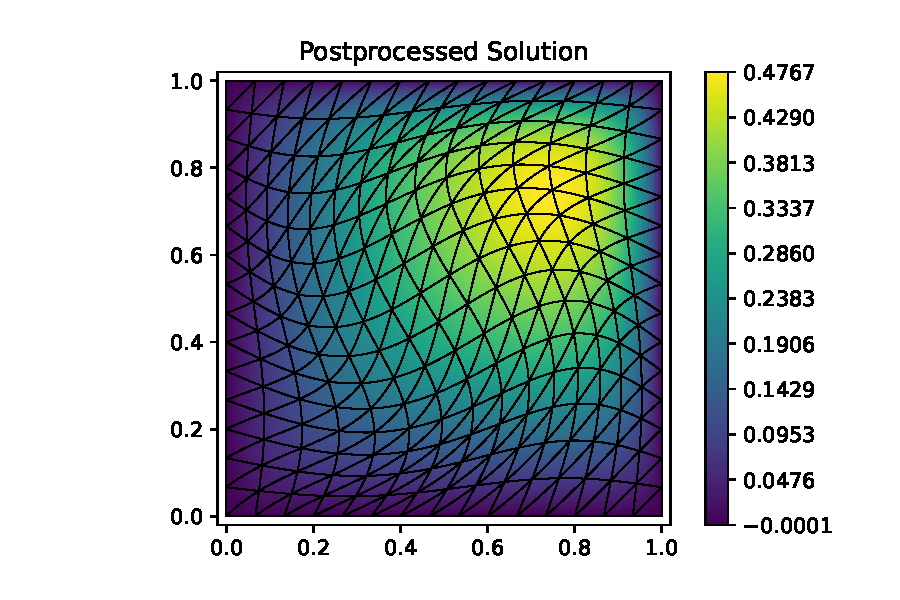
\includegraphics[width=0.5\textwidth]{ustarh_c_10_16.pdf}}
    \caption{$\mathbf{c}= (10,10)$}
    \label{f:conv_diff_2}
\end{figure}

\begin{figure}[H]
    \centering
    \subfloat[$u_h$.]{
        \label{f:square_straight}
        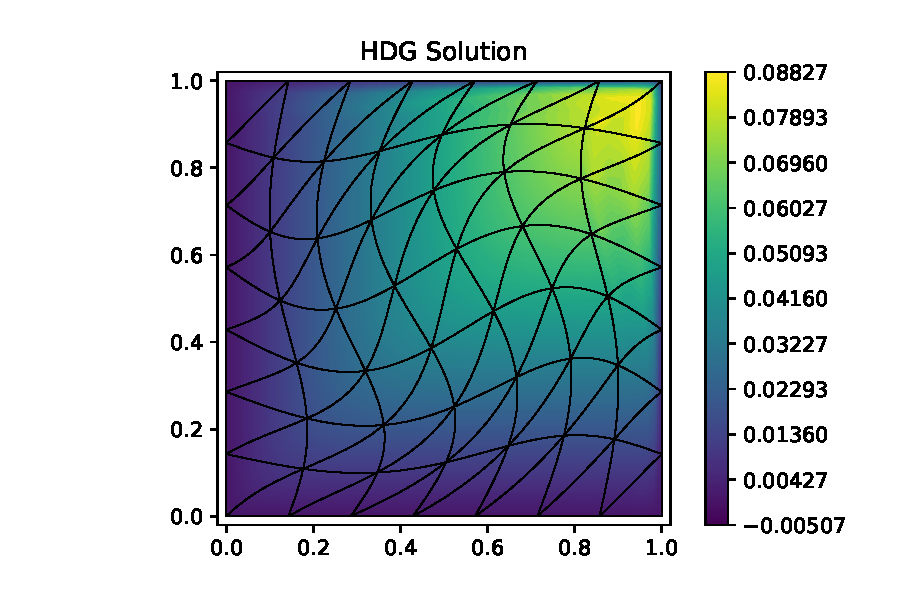
\includegraphics[width=0.5\textwidth]{uh_c_100_8.pdf}}
    \subfloat[$u^*_h$.]{
        \label{f:square_distorted}
        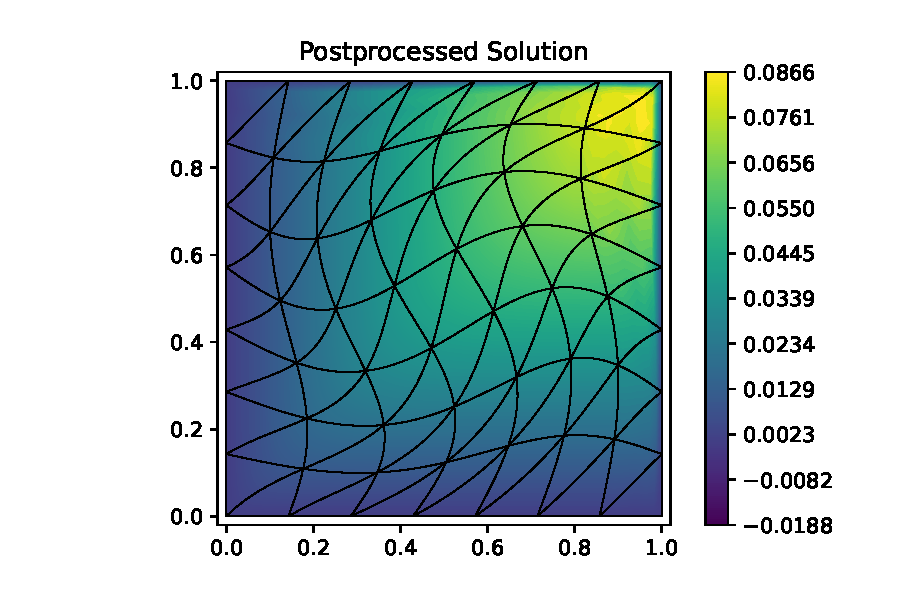
\includegraphics[width=0.5\textwidth]{ustarh_c_100_8.pdf}}\\
	\subfloat[$u_h$.]{
		\label{f:square_distorted}
		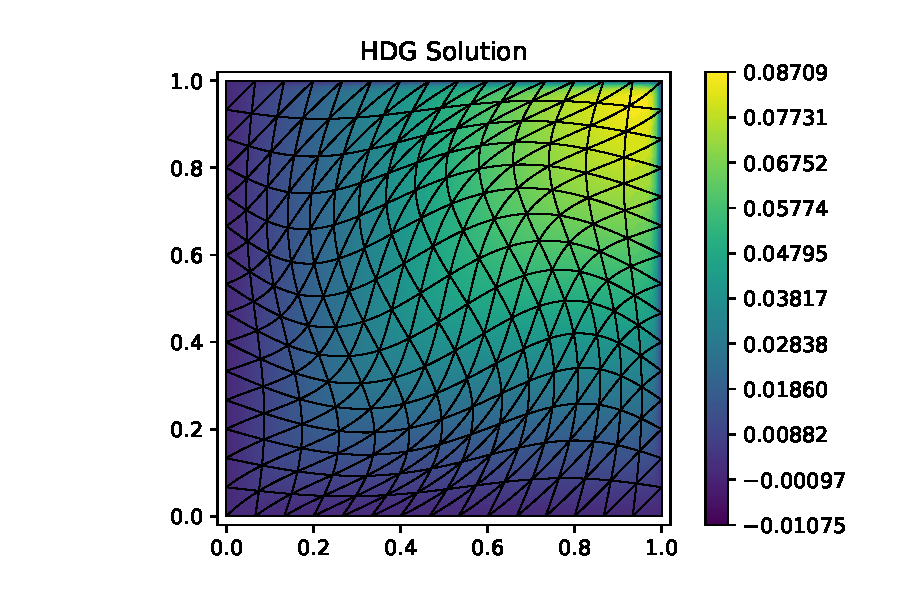
\includegraphics[width=0.5\textwidth]{uh_c_100_16.pdf}}
	\subfloat[$u^*_h$.]{
		\label{f:square_distorted}
		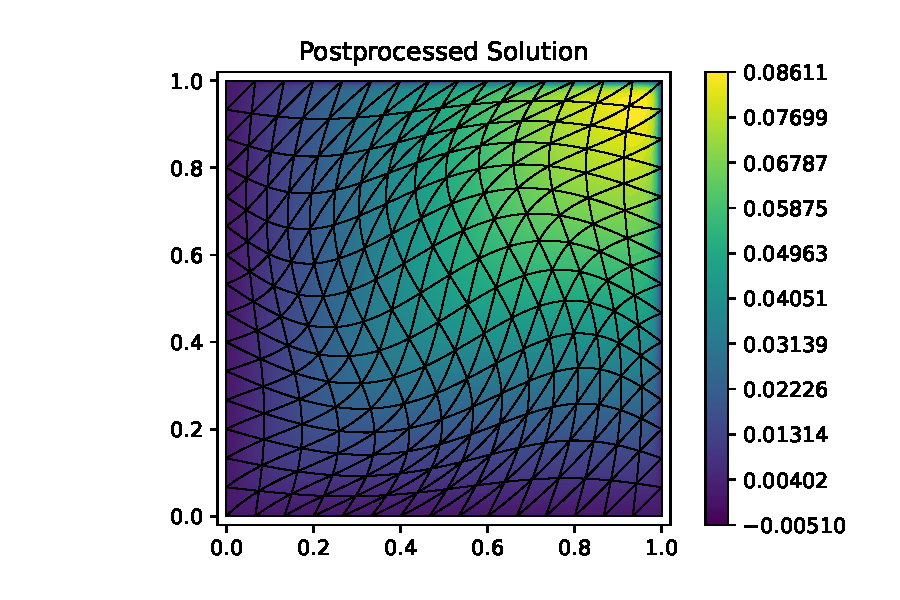
\includegraphics[width=0.5\textwidth]{ustarh_c_100_16.pdf}}\\
	\subfloat[$u_h$.]{
		\label{f:square_distorted}
		\includegraphics[width=0.5\textwidth]{uh_c_100_32.pdf}}
	\subfloat[$u^*_h$.]{
		\label{f:square_distorted}
		\includegraphics[width=0.5\textwidth]{ustarh_c_100_32.pdf}}
    \caption{$\mathbf{c}= (100,100)$}
    \label{f:conv_diff_3}
\end{figure}

It can be seen that the postprocessed solution is smoother than the solution coming directly from the HDG method, with this more noticeable in cases with coarse grids.
\section*{Final Project Proposal}

The main idea for the final project is to extend the code to solve the time-dependent 
1D Burgers Equation. The time-like variable will be treated as a second spatial dimension, and hence no need to
march the solution in time. However, since the equation is non-linear, a non-linear solver will have to be implemented.
After that, a point-wise sensor for shock capturing based on the entropy will be tested.
\subsection*{Add 1D Unsteady Inviscid Burgers Equation}

\begin{equation}
    \dfrac{\partial u}{\partial t} - \dfrac{\partial }{\partial x}\left(\dfrac{1}{2}u^2\right) = \alpha(x)u
\end{equation}
The source term might be needed to localize the shock and avoid a singular system.
\noindent
The idea is to solve the equation as a 2D steady problem, implementing also a non-linear solver.

\subsection*{Entropy Based Shock Sensor}

We motivate the idea by looking at the Burgers Equation with a thermoviscous difussion term:

\begin{equation}
    \dfrac{\partial u}{\partial t}
    -
    \dfrac{\partial}{\partial x}\left(\dfrac{1}{2}u^2\right)
    =
    \dfrac{\partial}{\partial x}\left(\dfrac{1}{\Gamma}\dfrac{\partial u}{\partial x}\right)
\end{equation}
Multiplying by $u$:

\begin{equation}
    u\dfrac{\partial u}{\partial t}
    -
    u\dfrac{\partial}{\partial x}\left(\dfrac{1}{2}u^2\right)
    =
    u\dfrac{\partial}{\partial x}\left(\dfrac{1}{\Gamma}\dfrac{\partial u}{\partial x}\right)
\end{equation}

\begin{equation}
    u\dfrac{\partial u }{\partial t}
    -
    u\dfrac{\partial}{\partial x}\left(\dfrac{1}{2}u^2\right)
    -
    \dfrac{\partial }{\partial x}\left(\dfrac{u}{\Gamma} \dfrac{\partial u}{\partial x}\right)
    =
    - \dfrac{1}{\Gamma}\left(\dfrac{\partial u}{\partial x}\right)^2 
    \leq 0
\end{equation}
From that, for the inviscid case:

\begin{equation}
    \eta
    :=
    u\dfrac{\partial u }{\partial t}
    -
    u\dfrac{\partial}{\partial x}\left(\dfrac{1}{2}u^2\right)
    \leq
    0
    \rightarrow \text{Entropy production}
\end{equation}
The hypothesis is that a shock will produce non-physical results, making $\eta > 0$ in the shock neighborhood.
So, we should add artificial viscosity where $\eta > 0$. The new PDE is:

\begin{equation}
    \dfrac{\partial u}{\partial t}
    -
    \dfrac{\partial}{\partial x}\left(\dfrac{1}{2}u^2\right)
    =
    \text{AV}(u,H)
\end{equation}

\begin{equation}
    u
    \left[
    \dfrac{\partial u}{\partial t}
    -
    \dfrac{\partial}{\partial x}\left(\dfrac{1}{2}u^2\right)
    \right]
    =
    u\text{AV}(u,H)
\end{equation}
We have to design $u\text{AV}(u,H)$ such that:

\begin{equation}
    u\text{AV}(u,H) \leq 0
\end{equation}
One option could be physical AV:

\begin{equation}
    \text{AV} = \dfrac{\partial }{\partial x}\left(\dfrac{1}{\Gamma_\text{AV}} \dfrac{\partial u}{\partial x}\right)
\end{equation}
and so:

\begin{equation}
    u\text{AV} 
    =
    u \dfrac{\partial }{\partial x}\left(\dfrac{1}{\Gamma_\text{AV}} \dfrac{\partial u}{\partial x}\right)
    =
    \dfrac{\partial}{\partial x}\left(\dfrac{u}{\Gamma_\text{AV}} \dfrac{\partial u}{\partial x}\right) - \dfrac{1}{\Gamma_\text{AV}}\left(\dfrac{\partial u}{\partial x}\right)^2
\end{equation}
All togheter:

\begin{equation}
    u
    \left[
    \dfrac{\partial u}{\partial t}
    -
    \dfrac{\partial}{\partial x}\left(\dfrac{1}{2}u^2\right)
    \right]
    =
    \dfrac{\partial}{\partial x}\left(\dfrac{u}{\Gamma_\text{AV}} \dfrac{\partial u}{\partial x}\right) - \dfrac{1}{\Gamma_\text{AV}}\left(\dfrac{\partial u}{\partial x}\right)^2
\end{equation}
We want:

\begin{equation}
    \dfrac{1}{\Gamma_\text{AV}}\left(\dfrac{\partial u}{\partial x}\right)^2
    >
    \eta^{+}
    \Rightarrow
    \dfrac{1}{\Gamma_\text{AV}}
    >\dfrac{\eta^+}{(\partial u/\partial x)^2}
    \label{e:gamma_condition}
\end{equation}
where we define:

\begin{equation}
	\eta^+ = \max(\eta,0)
\end{equation}
So, we can compute $\eta^+$ point-wise and add this artificial viscosity where needed.

\subsection*{In case of having extra time (unlikely)}

\subsubsection*{Solving for the Adjoint}

We could take advantage of the non-linear solver to also solve for 
the dual problem and get the adjoint solution. The final piece would be to implement an adjoint based error estimate, which should also take into account properly
the addition of artificial viscosity, which is not in the actual equation we are solving.

\end{document}